\section{Simulation study}
\label{sec:simulation}
\suppressfloats[t]
\subsection{Overview}
We separate two questions: whether a diagnostic describes expected CV bias, and whether it helps select an accurate CV estimate for an observed dataset. The second question also involves variation in the observed CV score between response datasets. Four experiments address these questions and examine how the answers depend on covariance estimation and the prediction model (Table~\ref{tab:studies}).

All primary comparisons use the four five-fold schemes in Section~\ref{sec:cv-selection}. Training locations are sampled uniformly or in clusters within the unit square. Targets cover either the same square or a square shifted horizontally by $0.5$, partly outside the sampled region. Total response variance is one. A simulation setting is one combination of sample size, covariance parameters, sampling pattern and target. The supplementary material (Section~\ref*{supp-sec:settings}) gives the complete designs.

\begin{table}[!htbp]
\centering\small
\caption{The four simulation experiments. Each scheme is evaluated on the same locations or responses within a repetition.}
\label{tab:studies}
\begin{tabular}{>{\raggedright\arraybackslash}p{3.1cm}>{\raggedright\arraybackslash}p{3.3cm}>{\raggedright\arraybackslash}p{7.0cm}}
\toprule
Experiment & Independent repetitions & Main outcome\\
\midrule
Known covariance & 5,120 location configurations & Exact MSE difference $O$; mean absolute expected bias after scheme selection\\
Estimated correlation & 1,440 datasets & Agreement between diagnostic signs and the sign of $O$\\
Covariance refitted within folds & 1,920 datasets & Mean absolute error of the selected CV score relative to conditional target MSE\\
Different prediction models & 480 simulated fields & Mean difference between target error and observed CV MSE\\
\bottomrule
\end{tabular}
\end{table}

Comparisons are paired within each repetition. Monte Carlo standard errors (MCSEs) use variation between independent repetitions within settings; folds and schemes are not counted as independent repetitions. Intervals of the form estimated difference $\pm1.96$ MCSE describe simulation uncertainty for the settings studied. Their calculation is given in the supplementary material (Section~\ref*{supp-sec:uncertainty}).

\subsection{Expected CV bias with known covariance}
\label{sec:sim-known}
\paragraph{Design.}
We first test whether correlation weighting helps choose a CV scheme when covariance is known. We vary sample size ($100$ or $250$), correlation scale $\phi$ ($0.05$ or $0.2$), signal fraction $w$ ($0$, $0.3$, $0.7$ or $0.95$), sampling pattern (uniform or clustered), target (within the sampled domain or shifted), and correlation family (exponential or Mat\'ern-$3/2$).

Combining these factors gives $2\times2\times4\times2\times2\times2=128$ settings. Each setting has 40 independent location configurations, giving $128\times40=5{,}120$ configurations in total. For each configuration, we draw a new sample of training locations and construct all four CV schemes. The 225-point target grid remains fixed within each setting.

For Gaussian prediction using all available training observations, expected CV MSE and target MSE are calculated exactly from the covariance matrices; no responses need to be simulated.

For each location configuration, each diagnostic rule selects among the same four CV schemes. We assess its choice by the absolute difference between expected CV MSE and target MSE, $|O|$. Table~\ref{tab:selection} and Figure~\ref{fig:reference}B average these differences across configurations. Smaller values mean that expected CV MSE is closer to the prediction MSE at the target locations.

We also assess whether $A$, $J_1$ and $J_2$ identify the sign of $O$, restricting this comparison to $|O|>0.01$, or more than 1\% of response variance. Correlation functions, configuration seeds, alternative thresholds and additional comparisons are in the supplementary material (Section~\ref*{supp-sec:known-details}).

\paragraph{Results.}
Selecting by $|J_2|$ reduced mean absolute expected bias from \BiasW\ under $W$ to \BiasJTwo, a \BiasReduction\% reduction. The paired difference was \BiasDelta\ (MCSE \BiasDeltaSE; Figure~\ref{fig:reference}B). The benefit varied with sampling pattern and target, and was small for uniform sampling with a target inside the sampled domain (Table~\ref{tab:selection}).

The sign of $J_2$ agreed with the sign of $O$ in \SignJTwo\% of eligible evaluations, compared with \SignJOne\% for $J_1$ and \SignA\% for $A$ (Figure~\ref{fig:reference}A). Known correlation therefore supplied useful information about both the direction and magnitude of expected bias, although no contrast identified the sign correctly in every case.

\begin{table}[!htbp]
\centering\small
\caption{Mean absolute expected bias, $|O|$, after scheme selection with known covariance. Smaller values mean that expected CV MSE is closer to the prediction MSE at the target locations. Each row averages 1,280 location configurations. Best of four averages the smallest true $|O|$ among the four candidates in each configuration. Fixed kNNDM uses kNNDM for every configuration. The last column is the paired difference for selection by $|J_2|$ minus selection by $W$, with its MCSE; negative values favour $|J_2|$.}
\label{tab:selection}
% Generated from the paired reference analysis.
\begin{tabular}{llrrrrr}
\toprule
Sampling & Target & \shortstack{Selection\\by $W$} & \shortstack{Selection\\by $|J_2|$} & \shortstack{Fixed\\kNNDM} & \shortstack{Best of\\four} & \shortstack{Difference\\(MCSE)} \\
\midrule
Uniform & In-domain & 0.0157 & 0.0155 & 0.0173 & 0.0153 & -0.00018 (0.00005) \\
Uniform & Shifted & 0.0777 & 0.0642 & 0.0766 & 0.0638 & -0.01352 (0.00052) \\
Clustered & In-domain & 0.0276 & 0.0240 & 0.0291 & 0.0234 & -0.00353 (0.00035) \\
Clustered & Shifted & 0.0428 & 0.0390 & 0.0495 & 0.0386 & -0.00383 (0.00031) \\
\bottomrule
\end{tabular}

\end{table}

\subsection{Reliability of contrasts with estimated covariance}
\label{sec:sim-covariance}
\paragraph{Design.}
The second experiment tests how estimating covariance or ignoring directional dependence affects the diagnostics. It uses 1,440 Gaussian response datasets with 160 observations each. Dependence is either isotropic, depending only on distance, or anisotropic, also depending on direction. We compare $J_2$ calculated using the true covariance, the true parameters with direction ignored, and an isotropic exponential covariance estimated from the responses. Under anisotropy, the true-covariance reference uses the most correlated training observation, which need not be the geographically nearest. The isotropic comparisons use the geographically nearest observation.

For each candidate CV scheme, expected bias is calculated using the true covariance. We use this reference to check whether $J_2$ calculated using estimated covariance identifies the direction of bias and whether values close to zero correspond to small bias. Section~\ref{sec:sim-refitting} tests the use of these contrasts for selecting a CV scheme. The supplementary material (Sections~\ref*{supp-sec:variogram} and~\ref*{supp-sec:covariance-diagnostics}) gives the fitting procedure and design.

\paragraph{Results.}
For evaluations with $|O|>0.01$, sign agreement fell from \SensIsoTrue\% with true covariance to \SensIsoEst\% with estimated covariance under isotropic dependence. Under directional dependence, agreement was \SensAnisoTrue\% with true covariance, \SensAnisoNominal\% when direction was ignored, and \SensAnisoEst\% with estimated isotropic covariance (Figure~\ref{fig:reference}C).

Even when $J_2$ calculated using estimated covariance was close to zero ($|J_2|\leq0.005$), expected CV MSE could differ substantially from prediction MSE at the target locations. Each evaluation considered one CV scheme on one dataset. Among evaluations meeting this threshold, the absolute MSE difference, $|O|$, exceeded $0.05$ in \SmallGapIso\% of isotropic cases and \SmallGapAniso\% of anisotropic cases (supplementary material, Section~\ref*{supp-sec:covariance-diagnostics}).

We obtained covariance estimates for all 1,440 datasets. Some estimated signal fractions were near zero or one, and some estimated correlation scales were much larger than the values used to generate the data (supplementary material, Section~\ref*{supp-sec:variogram} and Figure~\ref*{supp-fig:covariance-fits}).

Using true covariance, the bound in Equation~\ref{eq:certificate} contained every exact MSE difference but often included zero, leaving its sign unresolved. Smaller CV training sets also contributed to the error difference. The supplementary material (Section~\ref*{supp-sec:training-bound-results}) reports both calculations.

\subsection{Accuracy of CV estimates with fitted covariance}
\label{sec:sim-refitting}
\paragraph{Design.}
The third experiment evaluates scheme selection when covariance is estimated from responses. We combine correlation scales $0.05$ and $0.2$, signal fractions $0.3$, $0.7$ and $0.95$, uniform or clustered sampling, and targets within the sampled domain or shifted, giving $2\times3\times2\times2=24$ settings. Each setting has 80 independent datasets (1,920 in total), with 160 training and 225 target locations, exponential covariance and known mean zero.

Each CV fold uses its own covariance estimate, based only on its training responses, to predict the held-out observations. We separately estimate covariance from the full observed dataset for the final model's target predictions and the correlation contrasts used to select among the four schemes.

For each dataset, we use the known simulation model to calculate the final model's target MSE, $R_Q(Y_S)$. This averages over possible target responses while holding the observed training responses and fitted model fixed. We compare the selected CV score with this benchmark using $|R_Q(Y_S)-\widehat C|$. Averaging these absolute errors across datasets gives mean absolute error (MAE), so overestimates and underestimates cannot cancel. The supplementary material (Section~\ref*{supp-sec:refitting-scores}) gives the calculation and control comparisons.

\paragraph{Results.}
Across all 24 settings, selection by $|J_2|$ calculated using estimated covariance reduced MAE from \NestedMAEW\ under $W$ to \NestedMAEJTwo, a \NestedReduction\% reduction. The paired difference was \NestedDelta\ (MCSE \NestedSE; Monte Carlo interval \NestedLower\ to \NestedUpper; Figure~\ref{fig:reference}D). Both rules evaluate the same final model; the lower MAE means that selection by $|J_2|$ gave CV scores closer, on average, to its target MSE.

Almost all of the benefit came from one setting: uniform sampling, a shifted target, correlation scale $0.05$ and signal fraction $0.95$. In a post-hoc analysis, omitting that setting left a mean difference of \NestedOtherCellsDelta\ across the remaining 23 settings. Group comparisons, all omissions and scheme-selection frequencies are reported in the supplementary material (Section~\ref*{supp-sec:refitting-variation}).

A post-hoc check using ten folds on the same 1,920 datasets gave a 1.7\% MAE reduction for $|J_2|$ relative to $W$, but the Monte Carlo interval included zero. A separate paired comparison of five and ten folds could not establish whether using more folds changes the advantage of $|J_2|$ over $W$ (supplementary material, Section~\ref*{supp-sec:tenfold}).

\begin{figure}[p]
\centering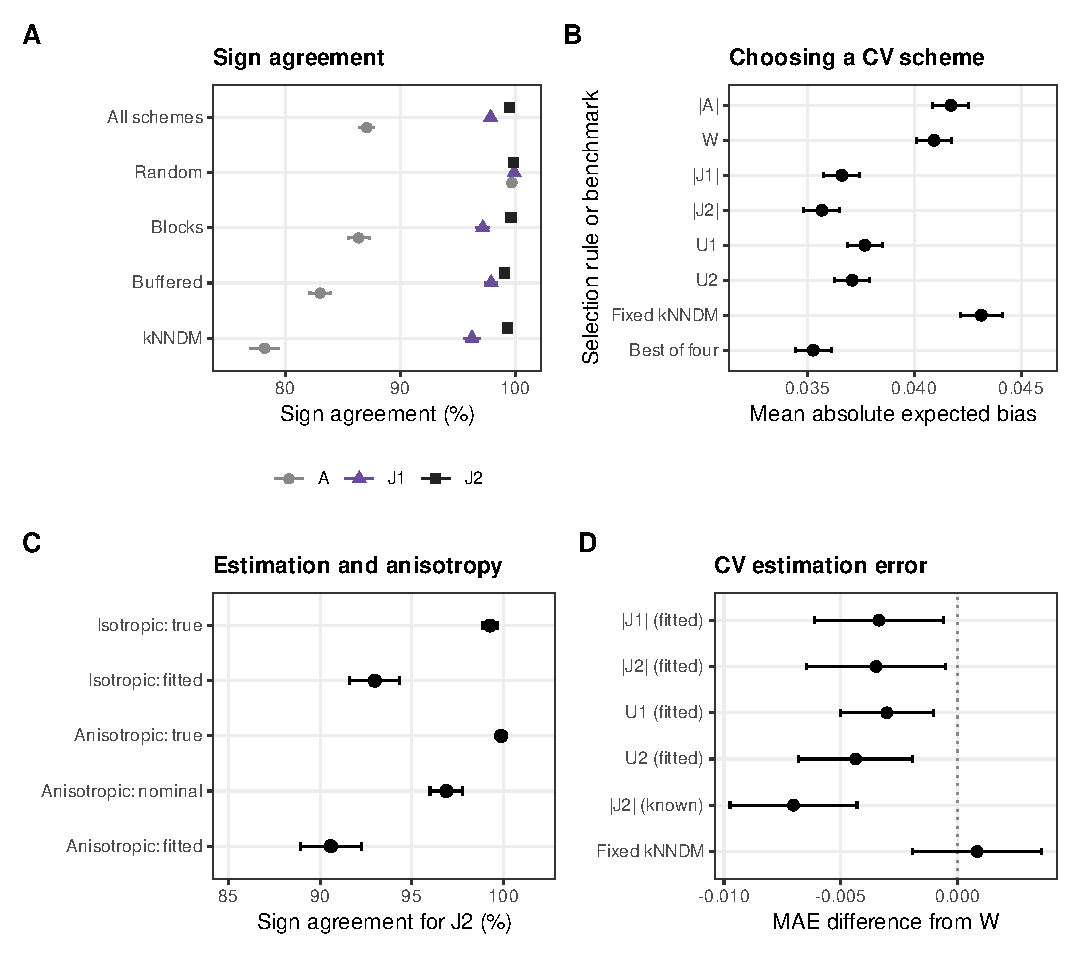
\includegraphics[width=\textwidth]{F2-reference.pdf}
\caption{Diagnostics under known and estimated covariance. Bars show $\pm1.96$ MCSE. (A) Sign agreement for $|O|>0.01$ under known covariance. (B) Mean absolute expected bias after selection. Smaller values mean that expected CV MSE is closer to the prediction MSE at the target locations. Best of four averages the smallest true $|O|$ among the four candidates in each configuration; fixed kNNDM uses kNNDM throughout. Fixed random CV gives \BiasRandom, outside the plotted scale. (C) Sign agreement using the true covariance, specified parameters with direction ignored (nominal), or estimated isotropic covariance (fitted). (D) Paired MAE differences relative to selection by $W$; negative values favour the listed rule. Prediction uses estimated covariance throughout D; \emph{known} refers only to the correlation weights used for selection.}
\label{fig:reference}
\end{figure}

\subsection{Dependence on the prediction model}
\label{sec:sim-learners}
\paragraph{Design.}
The fourth experiment tests whether CV bias can change while $J_1$ and $J_2$ remain fixed. These contrasts are differences between validation and target averages of correlations and squared correlations, respectively, with the nearest training observation (Section~\ref{sec:correlation-model}). Let $X$ and $Z$ be independent Gaussian fields with unit variance and the same exponential correlation. We observe $X$ as a predictor and generate responses using unobserved $Z$ and independent observation noise $\epsilon$:
\begin{equation}
 Y=\sqrt{\alpha}X+\sqrt{0.9-\alpha}Z+\epsilon,\qquad
 \alpha\in\{0,0.3,0.6,0.9\},\quad\Var(\epsilon)=0.1.
\end{equation}
Increasing $\alpha$ makes $X$ explain more response variation while reducing the contribution of unobserved $Z$. Total spatial variance remains $0.9$, so the response correlation before accounting for $X$ stays unchanged. With locations and folds fixed, $J_1$ and $J_2$ calculated from this correlation also remain unchanged.

Across 480 independent field configurations, we compare prediction using the known mean $\sqrt{\alpha}X$, linear regression on $X$, random forests on $X$ \citep{wright2017ranger}, inverse-distance weighting using coordinates, and kriging with known mean and residual covariance. Within each configuration, the fields, training noise and folds are reused across $\alpha$.

For each simulated field, \emph{target loss} is the average squared error against the noise-free target responses plus the observation-noise variance, $0.1$. We subtract observed CV MSE from this loss and average the differences across fields. Positive values mean that CV underestimates target MSE on average. The supplementary material (Section~\ref*{supp-sec:learner-details}) gives design and scoring details.

\begin{samepage}
\paragraph{Results.}
For random CV with clustered sampling, scale $0.2$ and a target inside the sampled domain, mean $J_2$ stayed at \ConstantMarginal. For the random forest, we averaged target loss minus CV MSE over the 60 simulated fields in this setting. This average fell from \ForestZero\ at $\alpha=0$ to \ForestNine\ at $\alpha=0.9$ (MCSEs \ForestZeroSE\ and \ForestNineSE): random CV underestimated target MSE much less when $X$ was more informative. For inverse-distance weighting, which does not use $X$, the average difference changed little: \IDWZero\ to \IDWNine\ (Figure~\ref{fig:learners}).

\end{samepage}

The known-mean model predicts $\sqrt{\alpha}X$ directly, using the true coefficient supplied by the simulation. Its remaining error is $\sqrt{0.9-\alpha}Z+\epsilon$, which has mean zero and variance $1-\alpha$ at every location. Expected CV and target MSE are therefore both $1-\alpha$, so expected CV bias is zero. At $\alpha=0.9$, the $Z$ term disappears. The remaining noise is independent between locations, so neighbouring responses cannot predict it. Kriging therefore also predicts $\sqrt{0.9}X$.

These comparisons show why $J_2$ based on response correlation alone cannot determine CV bias: it does not account for how a prediction model uses $X$. All settings and schemes are shown in the supplementary material (Figure~\ref*{supp-fig:learners-all}).

\begin{figure}[!htbp]
\centering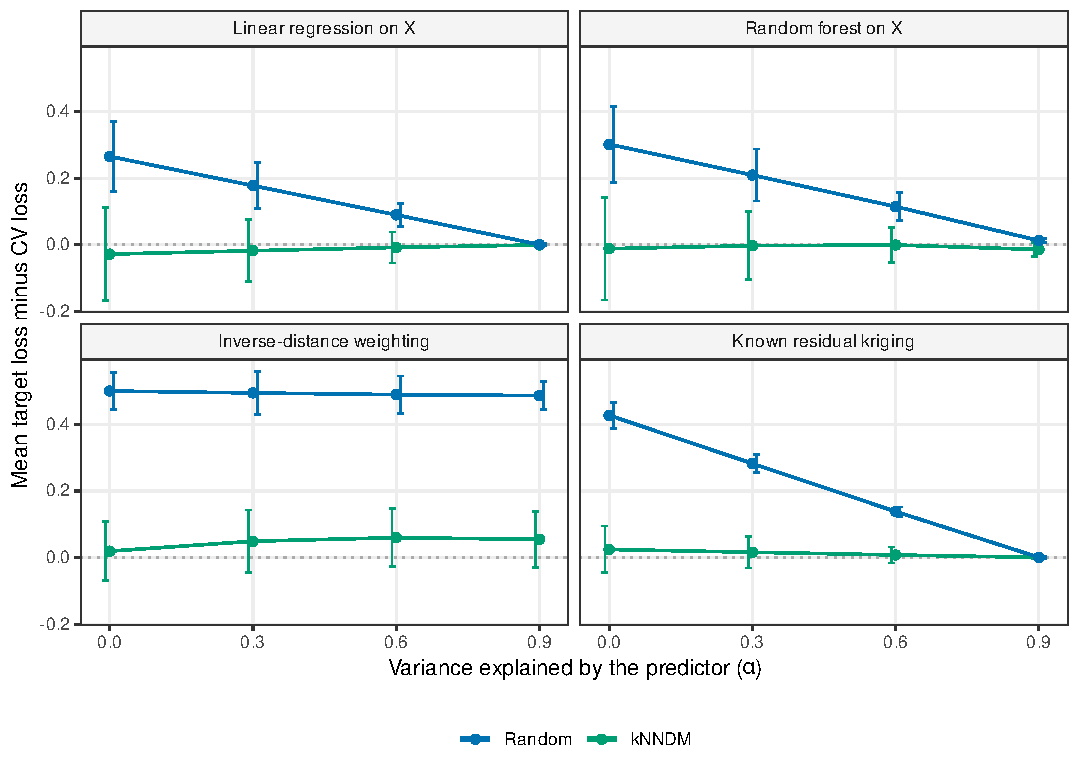
\includegraphics[width=\textwidth]{F3-learners.pdf}
\caption{CV bias changes as the predictor $X$ becomes more informative, while response correlation stays fixed. This setting uses clustered sampling, scale $0.2$ and a target inside the sampled domain. Points average target loss minus CV MSE over 60 fields; positive values mean that CV underestimates target MSE. Bars show $\pm1.96$ MCSE. The contrast $J_2$, calculated from response correlation before accounting for $X$, stays constant for each scheme, with random-CV mean \ConstantMarginal. Inverse-distance weighting uses coordinates alone. The supplementary material (Figure~\ref*{supp-fig:learners-all}) includes all settings and the known-mean model, whose expected CV bias is zero.}
\label{fig:learners}
\end{figure}
